% ============================================================
%  The Particle Model — Lesson Booklet (one section per lesson: A Reading · B Theory · C Practice · D Above level)
%  Year 7 (Year 8 extension)  |  Victorian Curriculum F–10 Version 2.0
%  Compile with: xelatex three times, then python3 fill.py Particle_Model_Lesson_Booklet_Yr7
% ============================================================
\documentclass[11pt,a5paper,twoside]{article}
\newcommand{\wrcoverfile}{../../../covers/ecosystems.jpg}\newcommand{\unitname}{Biodiversity and Ecosystems}\newcommand{\unitcaps}{BIODIVERSITY AND ECOSYSTEMS}

% ── Fonts (compile with LuaLaTeX) ────────────────────────────────────────────
\usepackage{fontspec}
% Bundled fonts (in ./fonts/) so the document compiles anywhere with XeLaTeX/LuaLaTeX
\setmainfont{Lato}[                   % body — humanist sans (stands in for deck's Inter)
  Path=../fonts/, Extension=.ttf, Ligatures=TeX,
  UprightFont=Lato-Regular, ItalicFont=Lato-Italic,
  BoldFont=Lato-Bold, BoldItalicFont=Lato-BoldItalic ]
\newfontfamily\headingfont{Poppins}[  % display/headings — matches the slide decks
  Path=../fonts/, Extension=.ttf, Ligatures=TeX,
  UprightFont=Poppins-Regular, ItalicFont=Poppins-Italic,
  BoldFont=Poppins-Bold, BoldItalicFont=Poppins-BoldItalic ]
\setlength{\headheight}{22pt}

\usepackage[protrusion=true,expansion=false]{microtype}
\usepackage[a5paper, inner=17mm, outer=13mm, top=19mm, bottom=17mm, headheight=14pt, headsep=4mm, footskip=8mm]{geometry}
\usepackage{xcolor}
\usepackage{tikz}
\usetikzlibrary{arrows.meta, shapes.geometric, calc, positioning, decorations.pathreplacing}
\usepackage{tcolorbox}
\tcbuselibrary{skins, breakable, raster}
\usepackage{fancyhdr}
\usepackage{titlesec}
\usepackage{enumitem}
\usepackage{booktabs}
\usepackage{tabularx}
\usepackage{array}
\usepackage{colortbl}
\usepackage{multicol}
\usepackage{amsmath}
\usepackage{needspace}
% TikZ diagram macros are embedded below (just before \begin{document}) for easy editing.
\usepackage{longtable}
\usepackage{graphicx}
\usepackage{pifont}
\usepackage{lastpage}
\usepackage{calc}
\usepackage{mdframed}
\usepackage{setspace}
\usepackage{ragged2e}
% PDF bookmarks: one per lesson (made in \sectiondiv) plus the cover and
% contents, and links from the contents table to each lesson.
% implicit=false: hyperref adds no anchors of its own (an anchor on each
% list item nudged lists down 1.5 mm, which would undo the page fill).
% hidelinks keeps the links invisible, so the printed pages are unchanged.
\usepackage[implicit=false, hidelinks,
  pdftitle={Biodiversity and Ecosystems — Lesson Booklet},
  pdfsubject={Years 7–8 Science, Victorian Curriculum F–10 v2.0}]{hyperref}
\usepackage{bookmark} % writes the outline itself, which implicit=false switches off in hyperref
% hyperref 7.01 with implicit=false leaves \Hy@PageAnchorSlide undefined, which
% throws at \end{document} and stops fill.py (it builds with -halt-on-error).
\makeatletter\providecommand\Hy@PageAnchorSlide{}\makeatother

% ── Colour Palette ───────────────────────────────────────────────────────────
% Remapped to the slide-deck palette (names kept so body + diagrams cascade)
\definecolor{NavyBlue}   {HTML}{16305C}
\definecolor{MidBlue}    {HTML}{2E6FE0}
\definecolor{LightBlue}  {HTML}{E8F1FF}
\definecolor{TealGreen}  {HTML}{0F6E63}
\definecolor{LightGreen} {HTML}{E0F7F3}
\definecolor{GoldDark}   {HTML}{C77F12}
\definecolor{GoldLight}  {HTML}{FFF3DC}
\definecolor{PurpleDark} {HTML}{5B3FC0}
\definecolor{PurpleLight}{HTML}{EFE9FF}
\definecolor{OrangeDark} {HTML}{C9483D}
\definecolor{OrangeLight}{HTML}{FFE9E6}
\definecolor{MidGrey}    {HTML}{AEBED4}
\definecolor{LightGrey}  {HTML}{F2F5FA}
\definecolor{DarkGrey}   {HTML}{3A4759}
\definecolor{TableHead}  {HTML}{16305C}
\definecolor{RowAlt}     {HTML}{EEF4FF}
% Bright accent tints (deck) for bars, rules and chips
\definecolor{Blue}   {HTML}{2E6FE0}
\definecolor{Teal}   {HTML}{18A999}
\definecolor{Amber}  {HTML}{F5A623}
\definecolor{Coral}  {HTML}{FF6B5E}
\definecolor{Violet} {HTML}{7C5CE0}
\definecolor{Sky}    {HTML}{4DA3FF}
\definecolor{Ink}    {HTML}{16223A}
\definecolor{Line}   {HTML}{DDE5F0}
\definecolor{Paper}  {HTML}{FBFCFE}

% ── Page Style ───────────────────────────────────────────────────────────────
\pagestyle{fancy}
\fancyhf{}
\renewcommand{\headrulewidth}{0.4pt}
\renewcommand{\headrule}{\hbox to\headwidth{\color{NavyBlue}\leaders\hrule height \headrulewidth\hfill}}
\fancyhead[L]{\headingfont\small\color{NavyBlue}The Particle Model}
\fancyhead[R]{\headingfont\small\color{DarkGrey}Year 7 \textbar{} Victorian Curriculum F--10 v2.0}
\fancyfoot[C]{\headingfont\small\color{DarkGrey}\thepage\ \textbar{} \pageref{LastPage}}
\fancypagestyle{plain}{%
  \fancyhf{}
  \fancyfoot[C]{\headingfont\small\color{DarkGrey}\thepage\ \textbar{} \pageref{LastPage}}
  \renewcommand{\headrulewidth}{0pt}
}

% ── Section Formatting ───────────────────────────────────────────────────────
\titleformat{\section}
  {\headingfont\color{NavyBlue}\Large\bfseries}
  {}{0em}{}
  [{\color{Teal}\rule[0.6ex]{2.2em}{3pt}}{\color{Line}\rule[0.6ex]{\dimexpr\linewidth-2.2em\relax}{1pt}}]
\titlespacing{\section}{0pt}{18pt}{8pt}

\titleformat{\subsection}
  {\headingfont\color{MidBlue}\large\bfseries}
  {\thesubsection}{0.6em}{}
\titlespacing{\subsection}{0pt}{12pt}{4pt}

\titleformat{\subsubsection}
  {\headingfont\color{NavyBlue}\normalsize\bfseries}
  {}{0em}{}
\titlespacing{\subsubsection}{0pt}{8pt}{2pt}

% Deck-style eyebrow / kicker (optional use)
\newcommand{\kicker}[2][Teal]{%
  {\headingfont\bfseries\footnotesize\color{#1}%
   \textcolor{#1}{\rule[0.18ex]{1.6em}{2.2pt}}\hspace{0.5em}\MakeUppercase{#2}\par}%
  \vspace{2pt}}

% ── Custom tcolorbox Environments ────────────────────────────────────────────

% Section divider banner
\newtcolorbox{sectionbanner}[2]{
  enhanced, breakable=false,
  colback=NavyBlue, colframe=NavyBlue,
  fontupper=\color{white}\bfseries\large,
  left=4mm, right=4mm, top=3mm, bottom=3mm,
  title={\color{white}\Huge\bfseries #1},
  attach boxed title to top left={yshift=-2mm, xshift=4mm},
  boxed title style={colback=NavyBlue, colframe=NavyBlue},
  after upper={\par\smallskip\normalfont\normalsize\color{white!80!NavyBlue}\textit{#2}}
}

% Key info box (blue)
\newtcolorbox{infobox}[1]{
  breakable, arc=2.5mm, boxrule=0.5pt,
  colback=LightBlue, colframe=Blue!40,
  fonttitle=\headingfont\bfseries, coltitle=MidBlue,
  title={#1},
  left=4mm, right=3.5mm, top=2.5mm, bottom=2.5mm
}

% Scaffold box (yellow)
\newtcolorbox{scaffold}[1]{
  breakable, arc=2.5mm, boxrule=0.5pt,
  colback=GoldLight, colframe=Amber!40,
  fonttitle=\headingfont\bfseries, coltitle=GoldDark,
  title={#1},
  left=4mm, right=3.5mm, top=2.5mm, bottom=2.5mm
}

% Worked example box
\newtcolorbox{workedexbox}[1]{
  breakable, arc=2.5mm, boxrule=0.5pt,
  colback=white, colframe=Amber!50,
  fonttitle=\headingfont\bfseries, coltitle=GoldDark,
  title={#1},
  left=4mm, right=3.5mm, top=2.5mm, bottom=2.5mm
}
% Worked examples: \begin{workedex}{title} -> "Worked Example N.M --- title",
% auto-numbered per section and labelled we:N.M. Never type the number.
\newcounter{wenum}[section]
\renewcommand{\thewenum}{\thesection.\arabic{wenum}}
\newenvironment{workedex}[1]
  {\refstepcounter{wenum}\label{we:\thewenum}\begin{workedexbox}{Worked Example \thewenum\ --- #1}}
  {\end{workedexbox}}

% We do: straight after each worked example, a near-identical question the
% class works through together, with its own writing space. Numbered to
% match the worked example above it and labelled wd:N.M.
%   \begin{wedo}{title} question ... \answerbox{h} \end{wedo}
\newtcolorbox{wedobox}[1]{
  enhanced, breakable=false, arc=2.5mm, boxrule=0.5pt,
  colback=white, colframe=TealGreen!55,
  fonttitle=\headingfont\bfseries, coltitle=TealGreen!75!black,
  title={#1},
  left=4mm, right=3.5mm, top=2.5mm, bottom=2.5mm
}
\newenvironment{wedo}[1]
  {\par\needspace{9\baselineskip}\begin{wedobox}{We do \thewenum\ --- #1}\label{wd:\thewenum}\ignorespaces}
  {\end{wedobox}}

% Year 7 box (blue)
\newtcolorbox{yr7box}{
  breakable, arc=2.5mm, boxrule=0.5pt,
  colback=LightBlue, colframe=Blue!40,
  left=4mm, right=3.5mm, top=2.5mm, bottom=2.5mm
}

% Year 8 extension box (violet)
\newtcolorbox{yr8box}{
  breakable, arc=2.5mm, boxrule=0.5pt,
  colback=PurpleLight, colframe=Violet!40,
  left=4mm, right=3.5mm, top=2.5mm, bottom=2.5mm
}

% Answer lines box
\newcommand{\answerbox}[1]{%
  \begin{tcolorbox}[
    enhanced, breakable, arc=2mm,
    colback=Paper, colframe=Line,
    left=2mm, right=2mm, top=1mm, bottom=1mm,
    boxrule=1pt,
    height=#1
  ]
  \end{tcolorbox}%
}

% Experiment header
\newtcolorbox{expheader}[3]{
  breakable=false, arc=2.5mm,
  colback=RowAlt, colframe=Amber!50, boxrule=0.5pt,
  fonttitle=\headingfont\bfseries\large, coltitle=NavyBlue,
  title={Experiment #1: #2},
  left=4mm, right=3.5mm, top=2.5mm, bottom=2.5mm,
  after upper={\par\smallskip
    {\headingfont\bfseries\color{GoldDark}Aim:}\ \textit{#3}},
}

% Reading comprehension passage box (green)
\newtcolorbox{readingbox}[1]{
  breakable, arc=2.5mm, boxrule=0.5pt,
  colback=white, colframe=Teal!50,
  fonttitle=\headingfont\bfseries, coltitle=TealGreen,
  title={#1},
  left=4mm, right=3.5mm, top=2.5mm, bottom=2.5mm,
  fontupper=\normalsize
}

% Skill-builder box (for beginner scaffolding)
\newtcolorbox{skillbox}[1]{
  breakable, arc=2.5mm, boxrule=0.5pt,
  colback=RowAlt, colframe=Blue!40,
  fonttitle=\headingfont\bfseries, coltitle=MidBlue,
  title={#1},
  left=4mm, right=3.5mm, top=2.5mm, bottom=2.5mm
}

% ── Custom Commands ───────────────────────────────────────────────────────────

% Question: \question{marks}{text}  (marks can be empty)
% Numbered automatically as Q<section>.<n>, reset every section.
% Do NOT write numbers by hand.
\newcounter{qnum}[section]
\renewcommand{\theqnum}{\thesection.\arabic{qnum}}
\newcommand{\question}[2]{%
  \refstepcounter{qnum}%
  \needspace{3\baselineskip}%
  \medskip
  \noindent\label{q:\theqnum}\textbf{Q\theqnum}\ifx&#1&\else\ \textcolor{DarkGrey}{(#1 mark\ifnum#1=1\else s\fi)}\fi\quad #2%
  \medskip
}

% Inline marks note
\newcommand{\markscount}[1]{\hfill\textcolor{DarkGrey}{\textit{(#1 mark\ifnum#1=1\else s\fi)}}}

% ── Practice set counter and question macros ─────────────────────────────────
\newcounter{pqnum}
\newcommand{\practiceset}[1]{%
  \needspace{6\baselineskip}
  \setcounter{pqnum}{0}%
  \vspace{6pt}
  {\headingfont\bfseries\large\color{GoldDark} Practice Set --- #1}\\[-2pt]
  {\color{Amber}\rule{\linewidth}{1pt}}\\[2pt]
}
% \pq{question text}{working box height}
\newcommand{\pq}[2]{%
  \stepcounter{pqnum}%
  \needspace{4\baselineskip}
  \vspace{5pt}
  \noindent\textbf{\thepqnum.}\quad #1\par
  \vspace{2pt}
  \answerbox{#2}
}
% Two short questions side by side, each with its own box
\newcommand{\pqpair}[4]{%
  \needspace{4\baselineskip}
  \vspace{5pt}
  \noindent
  \begin{minipage}[t]{0.48\linewidth}
    \stepcounter{pqnum}\textbf{\thepqnum.}\quad #1\par\vspace{2pt}
    \begin{tcolorbox}[enhanced,arc=2mm,colback=Paper,colframe=Line,left=2mm,right=2mm,
      top=1mm,bottom=1mm,boxrule=1pt,height=#2]\end{tcolorbox}
  \end{minipage}\hfill
  \begin{minipage}[t]{0.48\linewidth}
    \stepcounter{pqnum}\textbf{\thepqnum.}\quad #3\par\vspace{2pt}
    \begin{tcolorbox}[enhanced,arc=2mm,colback=Paper,colframe=Line,left=2mm,right=2mm,
      top=1mm,bottom=1mm,boxrule=1pt,height=#4]\end{tcolorbox}
  \end{minipage}
}

% ── Comprehension question macro (compact, lined) ────────────────────────────
\newcounter{rcnum}
\newcommand{\rcreset}{\setcounter{rcnum}{0}}
\newcommand{\rcq}[2]{%
  \stepcounter{rcnum}%
  \needspace{3\baselineskip}
  \vspace{4pt}
  \noindent\textbf{C\thercnum.}\quad #1\par
  \vspace{2pt}
  \linedbox{#2}
}

% Section divider (big numbered banner): \sectiondiv{title}{summary}
%
% This IS the section: it steps the real section counter, so subsections,
% tasks, questions and figures inside it are numbered N.M automatically.
% Put \label{sec:N} straight after it. Never hand-type a section number.
\newcommand{\sectiondiv}[2]{%
  \needspace{5\baselineskip}%
  \refstepcounter{section}%
  % PDF bookmark for the lesson; its anchor, lesson.N.1, is what the contents table links to
  \pdfbookmark[1]{Lesson \thesection{} — #1}{lesson.\thesection}%
  \begin{tcolorbox}[
    enhanced, breakable=false, arc=3.5mm,
    colback=NavyBlue, colframe=NavyBlue, boxrule=0pt,
    sidebyside, sidebyside align=center,
    lefthand width=2.4cm,
    left=2mm, right=4mm, top=4mm, bottom=4mm
  ]
    \begin{center}
      {\headingfont\bfseries\color{white!35!NavyBlue}\fontsize{50}{50}\selectfont \thesection}
    \end{center}
    \tcblower
    {\headingfont\bfseries\color{white}\LARGE #1}\\[3pt]
    {\itshape\color{white!75!NavyBlue}\small #2}
  \end{tcolorbox}%
}

% Tasks: \task, \task[a] (part a of a NEW task), \taskpart{b} (next part
% of the same task), \exttask (Year 8 "Extension" — same counter).
% Numbered Task <section>.<n>, reset every section. Do NOT type numbers.
% Every task, question and figure also gets an automatic label
% (task:1.7b, q:2.4, fig:1.2, fig:E2.1) so page refs come from the .aux.
\newcounter{tasknum}[section]
\renewcommand{\thetasknum}{\thesection.\arabic{tasknum}}
\NewDocumentCommand{\task}{o}{\refstepcounter{tasknum}\label{task:\thetasknum\IfValueT{#1}{#1}}\textbf{Task \thetasknum\IfValueT{#1}{#1}}}
\newcommand{\taskpart}[1]{\label{task:\thetasknum#1}\textbf{Task \thetasknum#1}}
\newcommand{\exttask}{\refstepcounter{tasknum}\label{task:\thetasknum}\textbf{Extension \thetasknum}}

% Figure captions: \figcap[fig:label]{caption} -> "Figure N.M --- caption"
% \expfigcap{caption} -> "Figure EN.M" (experiment pages). Both auto-numbered.
\newcounter{fignum}[section]
\renewcommand{\thefignum}{\thesection.\arabic{fignum}}
\newcounter{expfignum}[section]
\renewcommand{\theexpfignum}{E\thesection.\arabic{expfignum}}
\newcommand{\figcap}[2][]{%
  \begin{center}
    \refstepcounter{fignum}\label{fig:\thefignum}\if\relax\detokenize{#1}\relax\else\label{#1}\fi
    \small\itshape\color{DarkGrey} Figure \thefignum\ --- #2
  \end{center}%
}
\newcommand{\expfigcap}[1]{%
  \begin{center}
    \refstepcounter{expfignum}\label{fig:\theexpfignum}%
    \small\itshape\color{DarkGrey} Figure \theexpfignum\ --- #1
  \end{center}%
}

% Diagram include
\newcommand{\diagramfig}[3]{%  {filename}{width fraction}{caption}
  \begin{center}
    \includegraphics[width=#2\linewidth]{#1}\\[4pt]
    \small\itshape\color{DarkGrey} #3
  \end{center}%
}

% Table column types
\newcolumntype{L}[1]{>{\RaggedRight\arraybackslash}p{#1}}
\newcolumntype{C}[1]{>{\Centering\arraybackslash}p{#1}}

% Table header colour
\newcommand{\thead}[1]{\cellcolor{TableHead}\color{white}\bfseries #1}
\newcommand{\talt}{\rowcolor{RowAlt}}
\newcommand{\tmid}{\rowcolor{MidGrey}}

% Inline year tags
\newcommand{\tagyr}[1]{%
  \tikz[baseline=-0.5ex]\node[
    rounded corners=2pt,
    fill=#1!20, draw=#1, text=#1,
    inner xsep=4pt, inner ysep=1pt,
    font=\scriptsize\bfseries
  ]{Yr #1 only};}

% Draw answer lines
\newcommand{\anslines}[1]{%
  \vspace{2pt}%
  \foreach \n in {1,...,#1}{%
    \par\noindent\rule{\linewidth}{0.3pt}\vspace{3pt}%
  }%
}

% ── Document ─────────────────────────────────────────────────────────────────
% ── Optional-lesson note, shown under the lesson banner ──────────────────────
\newcommand{\optionalnote}[1]{%
  % the title is a bold lead-in on the first line rather than a title bar,
  % which keeps Lesson 11's reading on the lesson's first page
  \begin{tcolorbox}[enhanced, breakable=false, arc=2.5mm, boxrule=0.5pt,
    colback=PurpleLight, colframe=Violet!50,
    left=4mm, right=3.5mm, top=2mm, bottom=2mm]
  {\headingfont\bfseries\color{PurpleDark}Optional lesson \textbullet{} Year 8 extension.}\enspace #1
  \end{tcolorbox}\vspace{2pt}}


% ══════════════════════════════════════════════════════════════════════════════
%  LESSON STRUCTURE (lesson booklet, Oct 2026)
%  Every lesson runs in the same four parts, in this order:
%    \lessonpart{A}{Reading and comprehension}{Teal}   \label{read:N}
%    \lessonpart{B}{Theory and examples}{Blue}         \label{theory:N}
%    \lessonpart{C}{Practice}{Amber}                    \label{prac:N}
%    \lessonpart{D}{Above level}{Violet}                \label{ext:N}
%  Above-level / higher-order questions live ONLY in Part D, at the end.
% ══════════════════════════════════════════════════════════════════════════════
\newcommand{\lessonpart}[3]{%
  \par\if#1A\needspace{10\baselineskip}\vspace{10pt}\else
    \if#1C\notesfill\fi\clearpage\fi
  \begin{tcolorbox}[enhanced, breakable=false, arc=2mm, boxrule=0pt,
    colback=#3!14, borderline west={4pt}{0pt}{#3},
    left=4mm, right=3mm, top=1.6mm, bottom=1.6mm]
  {\headingfont\bfseries\color{#3!60!black}\large Part #1 \textbullet{} #2}
  \end{tcolorbox}\vspace{2pt}}

% Key vocabulary at the start of each lesson: students copy each definition
% from the vocabulary slide in the lesson's starter. First row = red scaffold.
\newcommand{\vocabhead}{%
  \par\vspace{6pt}%
  \begin{tcolorbox}[enhanced, breakable=false, arc=2mm, boxrule=0pt,
    colback=NavyBlue!10, borderline west={4pt}{0pt}{NavyBlue},
    left=4mm, right=3mm, top=1.6mm, bottom=1.6mm]
  {\headingfont\bfseries\color{NavyBlue}\large Key vocabulary}
  \end{tcolorbox}\vspace{2pt}%
  \noindent Copy the definition of each word from the slide. The first one has been done for you.\par}

% Curriculum codes under a lesson banner
\newcommand{\lessoncodes}[1]{%
  {\small\headingfont\color{DarkGrey}Victorian Curriculum 2.0:\ \textbf{#1}}\par\vspace{4pt}}

% Two short tasks side by side, each with its own working box
% \taskpair{text}{box height}{text}{box height}
% The two boxes line up: the shorter question is padded by the difference in
% text height (measured in a scratch box, task counter restored, no label).
\newsavebox\tpbox
\newlength\tpA \newlength\tpB
\newcount\tpsaved
\newcommand\tpmeasure[2]{%
  \tpsaved=\value{tasknum}%
  \sbox\tpbox{\vbox{\hsize=0.485\linewidth \linewidth=\hsize \parskip=0pt
    \renewcommand\label[1]{}\task #1\par}}%
  \setlength{#2}{\dimexpr\ht\tpbox+\dp\tpbox\relax}%
  \setcounter{tasknum}{\tpsaved}}
\newcommand{\taskpair}[4]{%
  \par\needspace{9\baselineskip}\vspace{4pt}%
  \tpmeasure{#1}{\tpA}\tpmeasure{#3}{\tpB}%
  \noindent
  \edef\abgrp{\number\numexpr\value{abox}+1\relax}%
  \begin{minipage}[t]{0.485\linewidth}
    \task #1\par\ifdim\tpB>\tpA\vspace{\dimexpr\tpB-\tpA\relax}\fi\vspace{2pt}\answerbox{#2}
  \end{minipage}\hfill
  \begin{minipage}[t]{0.485\linewidth}
    \task #3\par\ifdim\tpA>\tpB\vspace{\dimexpr\tpA-\tpB\relax}\fi\vspace{2pt}\answerbox{#4}
  \end{minipage}\par\gdef\abgrp{0}\vspace{4pt}}
% Two parts of one question side by side, with their answer boxes level:
% \ptpair{a}{part (a) text}{box height}{b}{part (b) text}{box height}.
% The shorter part's text gets space below it to match the longer one.
\newcommand\ptmeasure[3]{%
  \sbox\tpbox{\vbox{\hsize=0.485\linewidth \linewidth=\hsize \parskip=0pt \pt{#1}#2\par}}%
  \setlength{#3}{\dimexpr\ht\tpbox+\dp\tpbox\relax}}
\newcommand{\ptpair}[6]{%
  \ptmeasure{#1}{#2}{\tpA}\ptmeasure{#4}{#5}{\tpB}%
  \par\noindent
  \edef\abgrp{\number\numexpr\value{abox}+1\relax}%
  \begin{minipage}[t]{0.485\linewidth}
    \pt{#1}#2\par\ifdim\tpB>\tpA\vspace{\dimexpr\tpB-\tpA\relax}\fi\answerbox{#3}
  \end{minipage}\hfill
  \begin{minipage}[t]{0.485\linewidth}
    \pt{#4}#5\par\ifdim\tpA>\tpB\vspace{\dimexpr\tpA-\tpB\relax}\fi\answerbox{#6}
  \end{minipage}\par\gdef\abgrp{0}}

% Answer boxes never split across a page (a half box on its own page is useless)
% ── Page filling ────────────────────────────────────────────────────────────
% Every writing box gets an id. Its page is logged to \jobname.abp; fill.py
% measures the empty space left at the foot of each page and shares it out
% among that page's boxes via \jobname.abx (\abset{id}{extra}). Side-by-side
% boxes share a group so they grow together.
\newcounter{abox}
\newwrite\abpos \immediate\openout\abpos=\jobname.abp
\newcommand{\abset}[2]{\expandafter\gdef\csname abx@#1\endcsname{#2}}
\InputIfFileExists{\jobname.abx}{}{}
\def\abgrp{0}
\newcommand{\abnext}{\stepcounter{abox}%
  \edef\abcur{\ifcsname abx@\theabox\endcsname\csname abx@\theabox\endcsname\else 0pt\fi}}
\newcommand{\ablog}{\edef\abtmp{\noexpand\write\abpos{\theabox\space\abgrp\space\noexpand\thepage}}\abtmp}
\newcommand{\abh}[1]{\dimexpr#1+\abcur\relax}
\renewcommand{\answerbox}[1]{%
  \abnext
  \begin{tcolorbox}[enhanced, breakable=false, arc=2mm, colback=Paper, colframe=Line,
    left=2mm, right=2mm, top=1mm, bottom=1mm, boxrule=1pt, height=\abh{#1}]
  \end{tcolorbox}\ablog%
}
% \linedbox{height}: an answer box ruled in dotted thirds. Lines are \thirdrow/3 apart and run dotted, dotted,
% solid (the baseline), repeating, and end on one dotted line. The number of
% rows is worked out from the box's final height, so the ruling still fills the
% box after fill.py has grown it; the rows are centred in the box.
\newlength\thirdrow \setlength\thirdrow{9mm}
\tikzset{thirdsolid/.style={draw=DarkGrey!70, line width=0.5pt},
         thirddot/.style={draw=DarkGrey!70, line width=0.6pt, dash pattern=on 0.9pt off 1.6pt}}
\newlength\lbH \newlength\lbO \newcount\lbN
\newcommand{\linedbox}[1]{%
  \abnext
  % interior height = box height less the 1pt frame top and bottom
  \setlength\lbH{\dimexpr\abh{#1}-2pt\relax}%
  % whole rows that fit with at least 3 mm spare top and bottom (at least one)
  \lbN=\numexpr(\dimexpr\lbH-6mm-\thirdrow/2\relax)/\thirdrow\relax
  \ifnum\lbN<1 \lbN=1 \fi
  \setlength\lbO{\dimexpr(\lbH-\lbN\thirdrow)/2\relax}%
  \begin{tcolorbox}[enhanced, breakable=false, arc=2mm, colback=Paper, colframe=Line,
    left=2mm, right=2mm, top=1mm, bottom=1mm, boxrule=1pt, height=\abh{#1},
    underlay={\begin{tcbclipinterior}
      \foreach \i in {1,...,\the\lbN}{
        \draw[thirddot] ([xshift=3mm,yshift=-\lbO-(\i-1)*\thirdrow]interior.north west) -- ([xshift=-3mm,yshift=-\lbO-(\i-1)*\thirdrow]interior.north east);
        \draw[thirddot] ([xshift=3mm,yshift=-\lbO-(\i-1)*\thirdrow-\thirdrow/3]interior.north west) -- ([xshift=-3mm,yshift=-\lbO-(\i-1)*\thirdrow-\thirdrow/3]interior.north east);
        \draw[thirdsolid] ([xshift=3mm,yshift=-\lbO-(\i-1)*\thirdrow-2*\thirdrow/3]interior.north west) -- ([xshift=-3mm,yshift=-\lbO-(\i-1)*\thirdrow-2*\thirdrow/3]interior.north east);}
      \draw[thirddot] ([xshift=3mm,yshift=-\lbO-\lbN\thirdrow]interior.north west) -- ([xshift=-3mm,yshift=-\lbO-\lbN\thirdrow]interior.north east);
    \end{tcbclipinterior}}]
  \end{tcolorbox}\ablog%
}
% Every written-response box is ruled the same way (Part A comprehension, We do,
% Part C tasks and Part D extensions, including side-by-side pairs). Space for
% mathematical working uses \workbox{height} instead and stays plain, as do
% \drawbox and the write-in tables.
\let\workbox\answerbox   % plain box: mathematical working (calculations) stays unruled
\let\answerbox\linedbox
% \drawbox{height}{contents}: white box for a diagram or drawing
\newcommand{\drawbox}[2]{%
  \abnext
  \begin{tcolorbox}[colback=white, colframe=MidGrey, boxrule=0.5pt, height=\abh{#1}]#2\end{tcolorbox}\ablog}
% Notes box at the end of Part B: fills whatever is left of the page (if worth it)
\newcommand{\notesfill}{\par
  \ifdim\dimexpr\pagegoal-\pagetotal\relax>3.2cm
    \vspace*{\fill}%
    \begin{tcolorbox}[enhanced, breakable=false, arc=2mm, colback=Paper, colframe=Line,
      left=2mm, right=2mm, top=1mm, bottom=1mm, boxrule=1pt,
      height=\dimexpr\pagegoal-\pagetotal-1.0cm\relax]
      {\small\headingfont\color{DarkGrey}Notes}
    \end{tcolorbox}%
  \fi}



% Centred table: wrap every content table in \begin{ctab} ... \end{ctab}
% (figures already centre themselves inside their \diag... macros)
% ctab also registers write-in tables (S column) for page filling: the extra
% height is per row, logged with the row count.
\newenvironment{ctab}{\par\smallskip\begingroup\centering
  \abnext\let\tbcur\abcur\global\wtrows0 }{\par
  \ifnum\wtrows>0 \edef\abtmp{\noexpand\write\abpos{\theabox\space\abgrp\space\noexpand\thepage\space\the\wtrows}}\abtmp\fi
  \endgroup\smallskip}

% ── Booklet formatting rules (Oct 2026) ─────────────────────────────────────
% 1. No marks are shown anywhere in the booklet.
\renewcommand{\markscount}[1]{}
% 2. A task's heading sits on its own line; its text starts on the next
%    line, left aligned. Parts (a), (b)… each start a new line: use \pt{a}.
\RenewDocumentCommand{\task}{o}{\par\noindent\refstepcounter{tasknum}\label{task:\thetasknum\IfValueT{#1}{#1}}\textbf{Task \thetasknum\IfValueT{#1}{#1}}\par\nobreak\noindent\ignorespaces}
\renewcommand{\taskpart}[1]{\par\noindent\label{task:\thetasknum#1}\textbf{Task \thetasknum#1}\par\nobreak\noindent\ignorespaces}
\renewcommand{\exttask}{\par\noindent\refstepcounter{tasknum}\label{task:\thetasknum}\textbf{Extension \thetasknum}\par\nobreak\noindent\ignorespaces}
\newcommand{\pt}[1]{\par\noindent\textbf{(#1)}\ \ignorespaces}
% Workstation pages (Experiment 1): numbered method steps with a hanging
% indent, and a one-line safety reminder under the materials list.
\newcommand{\wsstep}[1]{\par\noindent\hangindent=1.6em\hangafter=1\makebox[1.6em][l]{\textbf{#1}}\ignorespaces}
\newcommand{\wssafety}[1]{\par\smallskip{\small\textcolor{ScaffoldRed}{\headingfont\bfseries Safety:}\ #1}\par}
% 3. Tables have vertical rules between columns and down both sides
%    (write | between and around the columns, e.g. {|L{3cm}|C{2cm}|}).
%    Keep the normal padding at the outer edges (no @{} there): colortbl paints
%    header colour one \tabcolsep past each edge, so trimming the padding makes
%    the header overhang the grid.
\arrayrulecolor{MidGrey}
\setlength{\arrayrulewidth}{0.6pt}
% 4. Write-in tables: W/Z are left/centred columns that centre text
%    vertically; put the S column first (see below).
\newcolumntype{W}[1]{>{\RaggedRight\arraybackslash}m{#1}}
\newcolumntype{Z}[1]{>{\Centering\arraybackslash}m{#1}}
\def\tbcur{0pt}
\newcount\wtrows
\newcommand{\wh}{\global\advance\wtrows1 \rule[\dimexpr-0.75cm-\tbcur/2\relax]{0pt}{\dimexpr1.5cm+\tbcur\relax}}
% S = zero-width first column that makes every row of a write-in table
% at least 1.5 cm tall with its text vertically centred. Start each data
% row with "&"; start the header row with "\hd &" so it stays slim.
\newif\ifnowh
\newcolumntype{S}{@{}>{}c<{\ifnowh\else\wh\fi\global\nowhfalse}@{\hspace{\tabcolsep}}}
\newcommand{\hd}{\global\nowhtrue}
% 5. The first row of a multi-row write-in table is a worked scaffold in red.
\definecolor{ScaffoldRed}{HTML}{C0392B}
\newcommand{\scaf}[1]{\textcolor{ScaffoldRed}{\itshape #1}}
% 6. Tables are a light grid (rules between rows and columns) on white —
%    row shading is off, because colortbl paints shading over column rules.
\renewcommand{\talt}{}
\renewcommand{\tmid}{}
% ══════════════════════════════════════════════════════════════════════════════
%  DIAGRAM DEFINITIONS — The Particle Model
%  Self-contained TikZ macros, no external image files. Each \diag... macro is
%  called from the body by name.
% ══════════════════════════════════════════════════════════════════════════════
\usetikzlibrary{arrows.meta,calc,positioning,patterns,backgrounds}
\tikzset{
  thin arrow/.style={-{Stealth[length=6pt,width=4pt]}, line width=1.4pt},
}

% ── Lesson 1: the same three jars holding a solid, a liquid and a gas ───────────
% The solid keeps its own shape, the liquid takes the jar's shape with a flat top,
% the gas fills the whole jar. No particles yet: those arrive in Lesson 4.
\newcommand{\jar}[1]{% jar outline with its base at (#1,0)
  \draw[line width=1.2pt, Ink] (#1-1.25,2.9) -- (#1-1.25,0.15) arc (180:270:0.15)
    -- (#1+1.1,0) arc (270:360:0.15) -- (#1+1.25,2.9);}
\newcommand{\diagStates}{%
\begin{center}
\begin{tikzpicture}[font=\small, x=1cm, y=1cm]
  % solid: a block sitting in the corner
  \fill[GoldLight] (-0.95,0.02) rectangle (0.15,1.25);
  \draw[GoldDark, line width=1.1pt] (-0.95,0.02) rectangle (0.15,1.25);
  \jar{0}
  \node[font=\bfseries, text=NavyBlue] at (0,-0.45) {Solid};
  \node[align=center, font=\footnotesize, text=DarkGrey] at (0,-1.05) {keeps its own shape\\and volume};
  % liquid: takes the jar's shape, flat top
  \begin{scope}[xshift=4.2cm]
    \fill[Sky!35] (-1.25,0.15) arc (180:270:0.15) -- (1.1,0) arc (270:360:0.15) -- (1.25,1.1) -- (-1.25,1.1) -- cycle;
    \draw[MidBlue, line width=1.1pt] (-1.25,1.1) -- (1.25,1.1);
    \jar{0}
    \node[font=\bfseries, text=NavyBlue] at (0,-0.45) {Liquid};
    \node[align=center, font=\footnotesize, text=DarkGrey] at (0,-1.05) {takes the jar's shape,\\keeps its volume};
  \end{scope}
  % gas: fills the whole (sealed) jar
  \begin{scope}[xshift=8.4cm]
    \fill[Violet!16] (-1.25,0.15) arc (180:270:0.15) -- (1.1,0) arc (270:360:0.15) -- (1.25,2.9) -- (-1.25,2.9) -- cycle;
    \draw[line width=2.2pt, DarkGrey] (-1.4,2.9) -- (1.4,2.9);
    \jar{0}
    \node[font=\scriptsize, text=DarkGrey, anchor=south] at (0,2.95) {lid};
    \node[font=\bfseries, text=NavyBlue] at (0,-0.45) {Gas};
    \node[align=center, font=\footnotesize, text=DarkGrey] at (0,-1.05) {spreads out to fill\\the whole jar};
  \end{scope}
\end{tikzpicture}
\end{center}}

% ── Lesson 1, Worked Example 1.2 and We do 1.2: the same syringe, before and after
\newcommand{\diagSyringe}[3]{% {start mL}{end mL}{contents: gas|liquid}
\begin{center}\resizebox{\linewidth}{!}{%
\begin{tikzpicture}[font=\scriptsize, x=0.11cm, y=1cm]
  \foreach \row/\vol/\lab in {0/#1/before, -1.15/#2/after}{
    \begin{scope}[yshift=\row cm]
      \ifx#3g\fill[Violet!16] (0,0) rectangle (\vol,0.7);\else\fill[Sky!35] (0,0) rectangle (\vol,0.7);\fi
      \draw[line width=1pt, Ink] (0,0) rectangle (60,0.7);
      \draw[line width=1pt, Ink] (0,0.25) -- (-4,0.25) (0,0.45) -- (-4,0.45);
      \fill[Ink] (-5.5,0.15) rectangle (-4,0.55);
      \foreach \t in {0,10,...,60}{\draw[Ink] (\t,0.7) -- (\t,0.85); \node[anchor=south, font=\tiny] at (\t,0.82) {\t};}
      \fill[DarkGrey] (\vol,0.04) rectangle (\vol+1.6,0.66);
      \draw[line width=2pt, DarkGrey] (\vol+1.6,0.35) -- (\vol+26,0.35);
      \draw[line width=2pt, DarkGrey] (\vol+26,0.05) -- (\vol+26,0.65);
      \node[anchor=east, font=\scriptsize\bfseries, text=DarkGrey] at (-7,0.35) {\lab};
    \end{scope}}
  \node[font=\tiny, text=DarkGrey, anchor=west] at (61,0.35) {mL};
  \node[font=\tiny, text=DarkGrey, anchor=north] at (-4.75,-1.2) {sealed tip};
\end{tikzpicture}}
\end{center}}

% needspace.sty reserves room by planting a penalty -100 with 9 lines of
% temporary stretch. On a page that can't be filled tightly that fake break
% always wins, so a We do that fitted was pushed over and left half a page
% empty. This version breaks only when the room really isn't there, and
% ragged bottom lets every other page run on until something won't fit;
% fill.py then grows the writing boxes into what is left at the foot.
\renewcommand{\needspace}[1]{\par\ifdim\dimexpr\pagegoal-\pagetotal\relax<\dimexpr#1\relax\newpage\fi}
\raggedbottom
% Part D sits in a breakable yr8box, where \needspace can't see the page (the box
% is built off the page first). Wrap each extension in keepext so it is one
% unsplittable block: the yr8box then breaks between extensions, never inside one.
\newenvironment{keepext}{\par\begin{tcolorbox}[blankest, breakable=false]}{\end{tcolorbox}\par}
\usetikzlibrary{patterns}
\providecommand{\lessonart}{\thesection}

\providecommand{\unitname}{Biodiversity and Ecosystems}\providecommand{\unitcaps}{BIODIVERSITY AND ECOSYSTEMS}
% ══════════════════════════════════════════════════════════════════════════════
%  2027 WORKBOOK STYLE — A5 LESSON BOOKLET (added by make_a5.py)
%  Same look as the Space A5 trial and the A4 experiment booklets: colour
%  cover, black-and-white inside, Outfit headings, a lesson opener band with
%  the lesson's ink symbol, boxes told apart by frame and icon:
%    I do ● solid · We do ●● dashed · You do ●●● heavy · key idea / reading ◆
%    thin · Above level ▲ double · Country ◎ dotted
%  The body still names the master's colours; they are mapped to ink here.
% ══════════════════════════════════════════════════════════════════════════════
\usepackage{pdflscape}
\usetikzlibrary{patterns}

% A picture wider than the A5 text block is scaled down to fit it.
\newsavebox\fitb
\newenvironment{fitbox}{\begin{lrbox}{\fitb}}{\end{lrbox}%
  \ifdim\wd\fitb>\linewidth\resizebox{\linewidth}{!}{\usebox\fitb}\else\usebox\fitb\fi}

% ── Fonts: Outfit for headings ──────────────────────────────────────────────
\renewfontfamily\headingfont{Outfit}[
  Path=../fonts/, Extension=.ttf, Ligatures=TeX,
  UprightFont=Outfit-Regular, BoldFont=Outfit-SemiBold,
  ItalicFont=Outfit-Regular, ItalicFeatures={FakeSlant=0.18},
  BoldItalicFont=Outfit-SemiBold, BoldItalicFeatures={FakeSlant=0.18} ]

% ── Black and white inside ──────────────────────────────────────────────────
\definecolor{Ink}{HTML}{111111}
\colorlet{NavyBlue}{Ink}\colorlet{MidBlue}{Ink}\colorlet{TealGreen}{Ink}
\colorlet{GoldDark}{Ink}\colorlet{PurpleDark}{Ink}\colorlet{OrangeDark}{Ink}
\colorlet{TableHead}{Ink}
\colorlet{Blue}{Ink}\colorlet{Teal}{Ink}\colorlet{Amber}{Ink}\colorlet{Coral}{Ink}
\colorlet{Violet}{Ink}\colorlet{Sky}{Ink}
\colorlet{LightBlue}{white}\colorlet{LightGreen}{white}\colorlet{GoldLight}{white}
\colorlet{PurpleLight}{white}\colorlet{OrangeLight}{white}\colorlet{RowAlt}{white}
\colorlet{LightGrey}{white}\colorlet{Paper}{white}
\colorlet{DarkGrey}{black!72}\colorlet{MidGrey}{black!45}\colorlet{Line}{black!45}
\arrayrulecolor{black!60}
% Particle kinds stay distinguishable without colour: white, light grey,
% dotted and dark.
\tikzset{
  pA/.style={circle, fill=white, draw=Ink, line width=0.6pt, minimum size=3.2mm, inner sep=0pt},
  pB/.style={circle, fill=black!35, draw=Ink, line width=0.6pt, minimum size=3.2mm, inner sep=0pt},
  pC/.style={circle, preaction={fill=white}, pattern=dots, draw=Ink, line width=0.6pt, minimum size=3.2mm, inner sep=0pt},
  pD/.style={circle, fill=black!75, draw=Ink, line width=0.6pt, minimum size=3.2mm, inner sep=0pt}}

% ── Page style: mirrored, running head on the outside ───────────────────────
\fancypagestyle{fancy}{\fancyhf{}%
  \renewcommand{\headrulewidth}{0.4pt}%
  \renewcommand{\headrule}{\hbox to\headwidth{\color{Ink}\leaders\hrule height \headrulewidth\hfill}}%
  \fancyhead[LE]{\headingfont\footnotesize \unitname}%
  \fancyhead[RO]{\headingfont\footnotesize\leftmark}%
  \fancyfoot[LE,RO]{\headingfont\footnotesize\thepage}}
\fancypagestyle{plain}{\fancyhf{}\renewcommand{\headrulewidth}{0pt}%
  \fancyfoot[LE,RO]{\headingfont\footnotesize\thepage}}
\fancypagestyle{opener}{\fancyhf{}\renewcommand{\headrulewidth}{0pt}%
  \fancyfoot[LE,RO]{\headingfont\footnotesize\thepage}}
\pagestyle{fancy}\markboth{}{}
\raggedbottom
\setlength{\emergencystretch}{2em}

\titleformat{\subsection}{\headingfont\large\bfseries}{\thesubsection}{0.6em}{}
\titleformat{\subsubsection}{\headingfont\normalsize\bfseries}{}{0em}{}

% ── Lesson opener band (replaces the navy section banner) ────────────────────
\renewcommand{\sectiondiv}[2]{%
  \clearpage\thispagestyle{opener}%
  \refstepcounter{section}\markboth{\thesection\ \textbullet\ #1}{\thesection\ \textbullet\ #1}%
  \pdfbookmark[1]{Lesson \thesection{} — #1}{lesson.\thesection}\hypertarget{lesson.\thesection.1}{}%
  \noindent\begin{minipage}[b]{\dimexpr\linewidth-36mm\relax}
    {\headingfont\bfseries\scriptsize\addfontfeatures{LetterSpace=14}\unitcaps\ \textbullet\ LESSON}\par\vspace{1mm}
    {\headingfont\bfseries\fontsize{40}{40}\selectfont\thesection}\par\vspace{1.5mm}
    {\headingfont\bfseries\fontsize{15}{18}\selectfont\RaggedRight #1\par}\vspace{1mm}
    {\footnotesize\itshape\RaggedRight #2\par}
  \end{minipage}\hfill
  \begin{minipage}[b]{34mm}\includegraphics[width=34mm]{../art/l\lessonart-ink.pdf}\end{minipage}\par
  \vspace{2.5mm}\noindent\rule{\linewidth}{1.6pt}\par\vspace{1mm}}
\renewcommand{\lessoncodes}[1]{{\small\itshape VC 2.0: #1}\par\vspace{2pt}}

% Lesson parts: a heading and a rule; B, C and D start a new page.
\renewcommand{\lessonpart}[3]{%
  \par\if#1A\needspace{10\baselineskip}\vspace{8pt}\else
    \if#1C\notesfill\fi\clearpage\fi
  {\headingfont\bfseries\Large Part #1 \textbullet\ #2}\par\vspace{0.5mm}\noindent\rule{\linewidth}{0.6pt}\par\vspace{1mm}}
\renewcommand{\vocabhead}{%
  \par\vspace{4pt}{\headingfont\bfseries\Large Key vocabulary}\par\vspace{1pt}%
  \noindent{\small Copy the meaning of each word from the slide. The first one has been done for you.}\par}
\renewcommand{\thead}[1]{\headingfont\bfseries #1}

% ── Box system ──────────────────────────────────────────────────────────────
\newcommand{\icodots}[1]{\tikz[baseline=-0.6ex]{\foreach \k in {1,...,#1}{\fill[white] (\k*1.9mm,0) circle (0.7mm);}}}
\newcommand{\icokey}{\tikz[baseline=-0.6ex]{\fill[white] (0,0.9mm)--(0.9mm,0)--(0,-0.9mm)--(-0.9mm,0)--cycle;}}
\newcommand{\icoup}{\tikz[baseline=-0.6ex]{\fill[white] (-1mm,-0.8mm)--(1mm,-0.8mm)--(0,1mm)--cycle;}}
\newcommand{\icocountry}{\tikz[baseline=-0.6ex]{\draw[white,line width=0.5pt] (0,0) circle (1mm); \fill[white] (0,0) circle (0.45mm);}}
\newcommand{\icoread}{\tikz[baseline=-0.6ex]{\draw[white,line width=0.6pt] (-1.1mm,-0.8mm) rectangle (1.1mm,0.8mm); \draw[white,line width=0.5pt] (0,-0.8mm) -- (0,0.8mm);}}
\newcommand{\tagicon}[1]{\tikz[baseline=-0.6ex]\node[fill=Ink, rounded corners=0.8mm, inner xsep=1.2mm, inner ysep=1mm]{#1};}
\tcbset{wbbase/.style={enhanced, colback=white, arc=1.2mm,
    left=3mm, right=3mm, top=4.2mm, bottom=2.4mm, before skip=10pt, after skip=7pt,
    attach boxed title to top left={xshift=3mm, yshift=-2.4mm},
    boxed title style={colback=Ink, colframe=Ink, arc=0.8mm, boxrule=0pt,
                       left=1.6mm, right=1.8mm, top=0.6mm, bottom=0.6mm},
    fonttitle=\headingfont\bfseries\footnotesize, coltitle=white}}
\renewtcolorbox{workedexbox}[1]{wbbase, breakable, colframe=Ink, boxrule=1pt,
  title={\icodots{1}\ I do \textbullet\ #1}}
\renewenvironment{workedex}[1]
  {\refstepcounter{wenum}\label{we:\thewenum}\begin{workedexbox}{Worked example \thewenum\ --- #1}}
  {\end{workedexbox}}
\renewtcolorbox{wedobox}[1]{wbbase, breakable=false, frame hidden,
  borderline={1.1pt}{0pt}{Ink, dash pattern=on 4pt off 2.6pt},
  title={\icodots{2}\ #1}}
\renewenvironment{wedo}[1]
  {\par\begin{wedobox}{We do \thewenum\ --- #1}\label{wd:\thewenum}\ignorespaces}
  {\end{wedobox}}
\renewtcolorbox{yr7box}{wbbase, breakable, colframe=Ink, boxrule=2.4pt, top=5mm,
  title={\icodots{3}\ You do \textbullet\ Check your understanding}}
\renewtcolorbox{yr8box}{wbbase, breakable, frame hidden,
  borderline={0.6pt}{0pt}{Ink}, borderline={0.6pt}{1.6pt}{Ink},
  title={\icoup\ Above level \textbullet\ Year 8 extension}}
\renewtcolorbox{infobox}[1]{wbbase, breakable, colframe=Ink, boxrule=0.5pt, title={\icokey\ #1}}
\renewtcolorbox{scaffold}[1]{wbbase, breakable, colframe=Ink, boxrule=0.5pt, title={\icokey\ #1}}
\renewtcolorbox{skillbox}[1]{wbbase, breakable, colframe=Ink, boxrule=0.5pt, title={\icokey\ #1}}
\renewtcolorbox{readingbox}[1]{wbbase, breakable, colframe=Ink, boxrule=0.5pt, title={\icoread\ #1}}
\renewtcolorbox{expheader}[3]{wbbase, breakable=false, colframe=Ink, boxrule=1pt,
  title={\icokey\ Experiment #1: #2},
  after upper={\par\smallskip{\headingfont\bfseries Aim:}\ \textit{#3}}}
\newtcolorbox{countrybox}[1]{wbbase, breakable, frame hidden,
  borderline={1.4pt}{0pt}{Ink, line cap=round, dash pattern=on 0pt off 2.4pt},
  title={\icocountry\ #1}}

% ── Padding to a multiple of 4 (copier booklet mode) ────────────────────────
\newcommand{\notespage}{\clearpage\markboth{Notes}{Notes}%
  {\headingfont\bfseries\Large Notes}\par\vspace{3mm}%
  \noindent\begin{tikzpicture}\foreach \y in {0,...,17}{\draw[black!35, line width=0.4pt] (0,-\y*9mm) -- (\linewidth,-\y*9mm);}\end{tikzpicture}}
\newcount\padleft
\newcommand{\padtofour}{\clearpage
  \pgfmathtruncatemacro\pagesused{\the\value{page}-1}%
  \pgfmathtruncatemacro\padn{mod(4-mod(\pagesused,4),4)}%
  \padleft=\padn\relax
  \loop\ifnum\padleft>0 \notespage\advance\padleft by -1 \repeat
  \clearpage}

% ══════════════════════════════════════════════════════════════════════════════
%  BIODIVERSITY AND ECOSYSTEMS — COVER
%  The unit's cover art (covers/ecosystems.jpg), full bleed. The A5 lesson
%  booklet sets \wrcoverfile one folder deeper.
% ══════════════════════════════════════════════════════════════════════════════
\providecommand{\wrcoverfile}{../../covers/ecosystems.jpg}
\newcommand{\wrcover}{%
\begin{tikzpicture}[remember picture, overlay]
  \node[anchor=north] at (current page.north) {\includegraphics[width=\paperwidth]{\wrcoverfile}};
\end{tikzpicture}}
% ── A5: every question full page width (stacked, never side by side) ───────
\renewcommand{\taskpair}[4]{%
  \par\needspace{6\baselineskip}\vspace{2pt}%
  \task #1\par\vspace{2pt}\answerbox{#2}%
  \par\needspace{6\baselineskip}%
  \task #3\par\vspace{2pt}\answerbox{#4}\par\vspace{2pt}}
\renewcommand{\ptpair}[6]{%
  \pt{#1}#2\par\answerbox{#3}%
  \pt{#4}#5\par\answerbox{#6}}
\renewcommand{\pqpair}[4]{%
  \needspace{4\baselineskip}\vspace{5pt}%
  \stepcounter{pqnum}\noindent\textbf{\thepqnum.}\quad #1\par\vspace{2pt}
  \begin{tcolorbox}[enhanced,arc=2mm,colback=Paper,colframe=Line,left=2mm,right=2mm,
    top=1mm,bottom=1mm,boxrule=1pt,height=#2]\end{tcolorbox}
  \stepcounter{pqnum}\noindent\textbf{\thepqnum.}\quad #3\par\vspace{2pt}
  \begin{tcolorbox}[enhanced,arc=2mm,colback=Paper,colframe=Line,left=2mm,right=2mm,
    top=1mm,bottom=1mm,boxrule=1pt,height=#4]\end{tcolorbox}}

\begin{document}
\pdfbookmark[1]{Cover}{cover}
\setlength{\parindent}{0pt}
\setlength{\parskip}{4pt}

% ---- Cover: the unit's cover art, full bleed, in colour ------------------
\thispagestyle{empty}
\begin{tikzpicture}[remember picture, overlay]
  \node[anchor=north] at (current page.north) {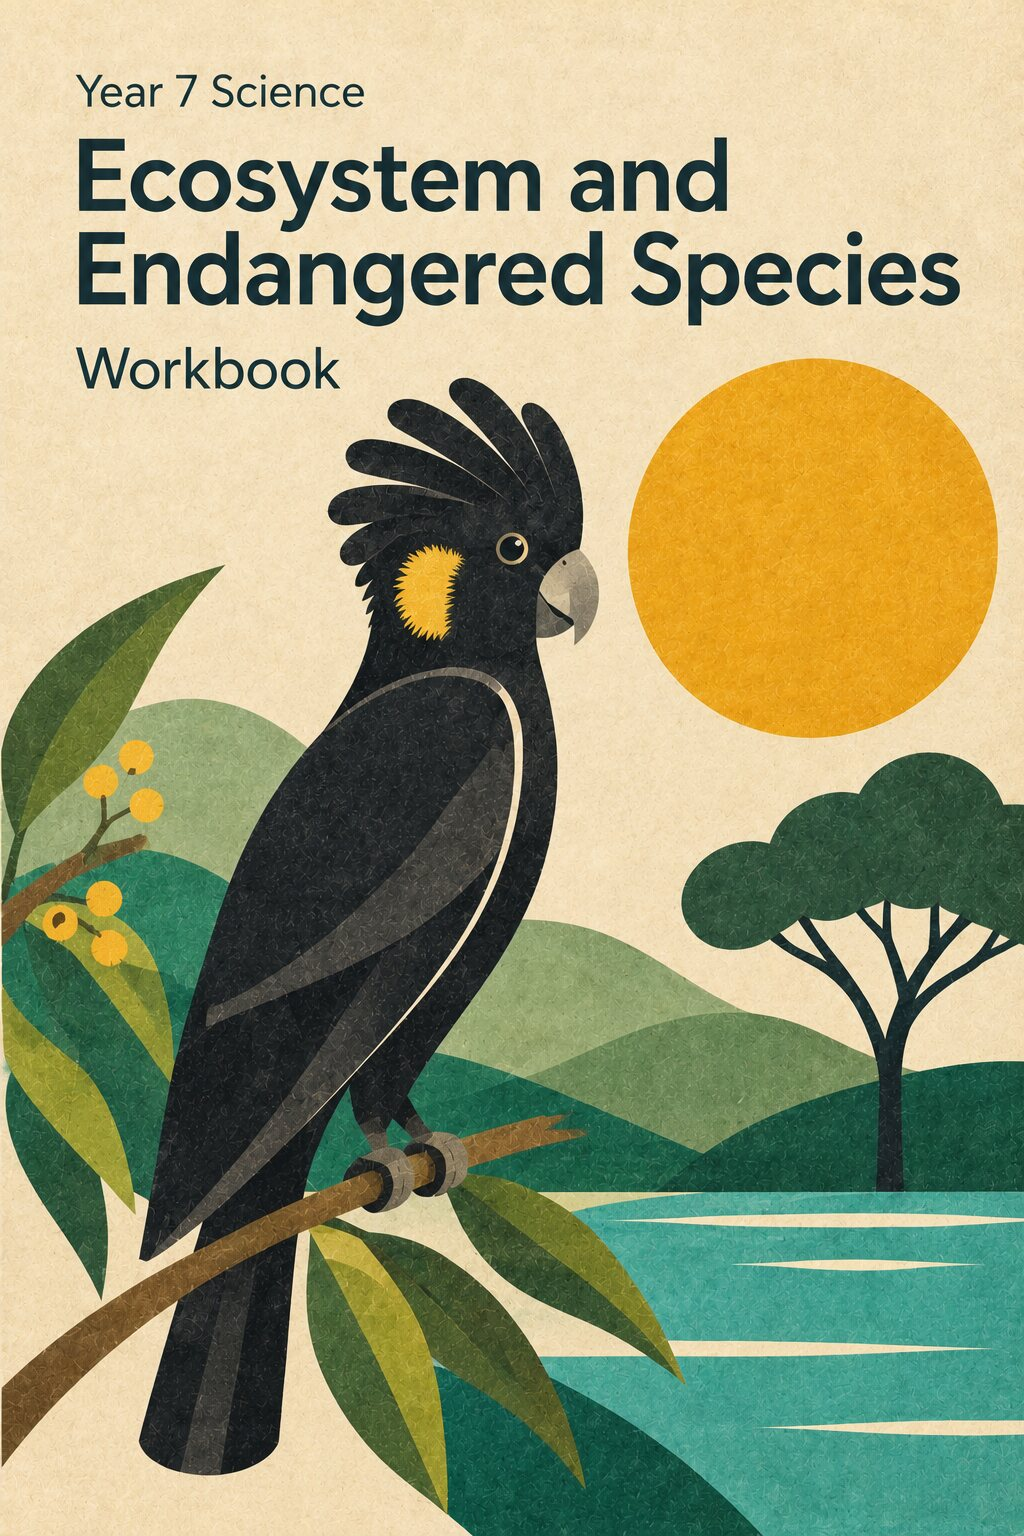
\includegraphics[width=\paperwidth]{../../../covers/ecosystems.jpg}};
  \node[anchor=north east, fill=white, draw=Ink, line width=0.6pt, rounded corners=1.2mm,
        inner xsep=2mm, inner ysep=1.8mm, text width=30mm, font=\headingfont\footnotesize]
    at ([xshift=-4mm, yshift=-4mm]current page.north east)
    {\textbf{Name}\par\vspace{4mm}\hrule\vspace{2mm}\textbf{Class}\par\vspace{4mm}\hrule};
  \node[anchor=south east, fill=white, draw=Ink, line width=0.6pt, rounded corners=1.2mm,
        inner xsep=2.6mm, inner ysep=2mm, font=\headingfont\bfseries, align=right]
    at ([xshift=-4mm, yshift=6mm]current page.south east)
    {Lesson Booklet 1\\[-1pt]{\normalfont\headingfont\scriptsize Lessons 1--4}};
\end{tikzpicture}
\mbox{}
\clearpage

% ---- Inside cover ---------------------------------------------------------
\thispagestyle{plain}
{\headingfont\bfseries\fontsize{22}{26}\selectfont Biodiversity and Ecosystems}\par\vspace{1mm}
{\headingfont\large Lesson Booklet 1 \textbullet\ Lessons 1--4 \textbullet\ Year 7}\par\vspace{1mm}
{\small\itshape VC 2.0: VC2S8U01 \textbullet\ VC2S8U04 \textbullet\ VC2S8I01--I08 \textbullet\ VC2S8H02--H04}\par\vspace{4mm}
\textbf{Teacher}\ \hrulefill\par

\begin{countrybox}{Acknowledgement of Country}
This booklet was created on the unceded Country of the Wurundjeri Woi-wurrung people of the Kulin Nation. We acknowledge Elders past, present and emerging.
\end{countrybox}

\begin{infobox}{How this booklet works}
One section for each lesson. Each opens with its key vocabulary, then:\par\smallskip
\renewcommand{\arraystretch}{1.25}
\begin{tabular}{@{}p{24mm}p{70mm}@{}}
\textbf{Part A} & a reading with comprehension questions \\
\textbf{Part B} & the ideas, worked through \\
\textbf{Part C} & practice on your own \\
\end{tabular}

\smallskip
\begin{tabular}{@{}p{24mm}p{70mm}@{}}
\textbf{I do} \tagicon{\icodots{1}} & your teacher works an example (solid frame) \\
\textbf{We do} \tagicon{\icodots{2}} & you try one together (dashed frame) \\
\textbf{Reading} \tagicon{\icoread} & a passage to read (thin frame) \\
\end{tabular}

\smallskip
Three lesson books. The five labs share a lesson and are in the \textbf{Experiment Booklet}. Finished your lesson work and want to go further? Ask your teacher about \textbf{Advanced Ecosystems}.
\end{infobox}

\clearpage
\markboth{Contents}{Contents}
{\headingfont\bfseries\LARGE Contents}\par\vspace{1mm}\noindent\rule{\linewidth}{0.6pt}\par\vspace{2mm}
\renewcommand{\arraystretch}{1.45}
\begin{tabular}{|C{1.1cm}|L{6.0cm}|C{2.4cm}|}
  \hline\thead{Lesson} & \thead{Title} & \thead{Page} \\ \hline
  1 & \hyperlink{lesson.1.1}{Living or Non-living?} \newline{\footnotesize\itshape + Lab: Is Yeast Alive? (Experiment Booklet)} & \hyperlink{lesson.1.1}{p.\ \pageref{sec:1}} \\ \hline
  2 & \hyperlink{lesson.2.1}{Classification: Linnaean Levels} & \hyperlink{lesson.2.1}{p.\ \pageref{sec:2}} \\ \hline
  3 & \hyperlink{lesson.3.1}{Scientific Names and the Six Kingdoms} & \hyperlink{lesson.3.1}{p.\ \pageref{sec:3}} \\ \hline
  4 & \hyperlink{lesson.4.1}{Dichotomous Keys} \newline{\footnotesize\itshape + Lab: Key the Schoolyard (Experiment Booklet)} & \hyperlink{lesson.4.1}{p.\ \pageref{sec:4}} \\ \hline
  5 & \textit{Australian Ecosystems and Biodiversity} \newline{\footnotesize\itshape + Lab: Quadrat Survey (Experiment Booklet)} & Book 2 \\ \hline
  6 & \textit{Food Webs and Energy Flow} & Book 2 \\ \hline
  7 & \textit{Ecosystem Services} & Book 2 \\ \hline
  8 & \textit{Adaptations} \newline{\footnotesize\itshape + Lab: Beaks and Food (Experiment Booklet)} & Book 2 \\ \hline
  9 & \textit{Introduced Species} \newline{\footnotesize\itshape + Lab: The Rabbit and Fox Model (Experiment Booklet)} & Book 3 \\ \hline
  10 & \textit{Human Impacts on Ecosystems} & Book 3 \\ \hline
  11 & \textit{Conservation and Action} & Book 3 \\ \hline
  --- & \hyperlink{glossary}{Glossary} & \hyperlink{glossary}{\pageref{sec:glossary}} \\ \hline
\end{tabular}
\renewcommand{\arraystretch}{1}
\clearpage
% ══════════════════════════════════════════════════════════════════════════════
%  BIODIVERSITY AND ECOSYSTEMS — A5 LESSON BOOKLET, LESSONS 1–4
%  Written for the 2027 workbook style from Bio_Ecosystems_Unit_Booklet_Yr7_8.tex
%  (same ideas, tasks and First Nations content; restructured into Parts A–D).
%  Built by make_a5.py. Lesson numbers = the unit's planner (planner-data.json).
% ══════════════════════════════════════════════════════════════════════════════

% ══════════════════════════════════════════════════════════════════════════════
%  LESSON 1 — LIVING OR NON-LIVING?
% ══════════════════════════════════════════════════════════════════════════════
\setcounter{section}{0}
\sectiondiv{Living or Non-living?}{MRS GREN \textbullet{} The seven life processes \textbullet{} Dead versus never alive}\label{sec:1}
\lessoncodes{VC2S8U01 \textbullet{} VC2S8H02}

\vocabhead
\begin{ctab}
\begin{tabular}{|SW{3.4cm}|W{7.0cm}|}
  \hline\hd & \thead{Word} & \thead{Definition (copy from the slide)} \\ \hline
  & \scaf{\textbf{Organism}\label{voc:organism}} & \scaf{A single living thing, such as a plant, an animal, a fungus or a bacterium.} \\ \hline
  & \textbf{Life process}\label{voc:life-process} & \\ \hline
  & \textbf{Respiration}\label{voc:respiration} & \\ \hline
  & \textbf{Excretion}\label{voc:excretion} & \\ \hline
  & \textbf{Sensitivity}\label{voc:sensitivity} & \\ \hline
  & \textbf{Cell}\label{voc:cell} & \\ \hline
\end{tabular}
\end{ctab}

% ─── PART A ───────────────────────────────────────────────────────────────────
\lessonpart{A}{Reading and comprehension}{Teal}\label{read:1}

\begin{readingbox}{Reading --- What Makes Something Alive?}
A kangaroo is alive. A rock is not. That much is easy. But what about a seed that has sat in a packet for five years, a mushroom, or a flame that seems to eat, breathe and grow?

Scientists decide whether an \textbf{organism} is alive by checking for seven \textbf{life processes}. Every living thing carries out all seven, at least at some point in its life. They are remembered with the name \textbf{MRS GREN}: Movement, Respiration, Sensitivity, Growth, Reproduction, Excretion and Nutrition.

Some of these are easy to see. A possum moves, grows and has young. Others happen out of sight. \textbf{Respiration} is a chemical reaction in every cell that releases energy from food. \textbf{Excretion} is getting rid of the waste that the body's chemical reactions make. \textbf{Sensitivity} is detecting changes around you and responding to them: a plant bends towards light, and a lizard runs from a shadow.

There is one more test. Every living thing is made of one or more \textbf{cells}, the tiny building blocks of life. A thing that was once alive, like a dry leaf or a wooden desk, is \emph{dead}. A thing that was never alive, like a river rock, is \emph{non-living}.
\end{readingbox}

\rcreset
\rcq{What does each letter of MRS GREN stand for?}{2.5cm}
\rcq{What is respiration, and where does it happen?}{2.5cm}
\rcq{Give an example of sensitivity in a plant and in an animal.}{2.5cm}
\rcq{What is the difference between \emph{dead} and \emph{non-living}?}{2.5cm}
\rcq{What are all living things made of?}{1.5cm}

% ─── PART B ───────────────────────────────────────────────────────────────────
\lessonpart{B}{Theory and examples}{Blue}\label{theory:1}

\subsection{The Seven Life Processes}\label{sub:1.1}

\begin{center}
\begin{fitbox}\begin{tikzpicture}[font=\small,
  lp/.style={draw=Ink, line width=0.7pt, rounded corners=1.2mm, fill=white, minimum width=2.5cm, minimum height=0.75cm, align=center}]
  \node[draw=Ink, line width=1.2pt, circle, minimum size=1.9cm, font=\headingfont\bfseries, align=center] (c) at (0,0) {MRS\\GREN};
  \foreach \a/\t [count=\i] in {90/{\textbf{M}ovement}, 38.6/{\textbf{R}espiration}, -12.9/{\textbf{S}ensitivity}, -64.3/{\textbf{G}rowth}, -115.7/{\textbf{R}eproduction}, -167.1/{\textbf{E}xcretion}, 141.4/{\textbf{N}utrition}}{
    \node[lp] (n\i) at (\a:2.75) {\t};
    \draw[Ink, line width=0.6pt] (c) -- (n\i);}
\end{tikzpicture}\end{fitbox}
\figcap{The seven life processes.}
\end{center}

\begin{skillbox}{MRS GREN}
\renewcommand{\arraystretch}{1.15}
\begin{tabular}{@{}p{2.4cm}p{7.3cm}@{}}
\textbf{Movement} & All living things move in some way; even plants move slowly towards light. \\
\textbf{Respiration} & Releasing energy from food, inside every cell. \\
\textbf{Sensitivity} & Detecting changes in the surroundings and responding to them. \\
\textbf{Growth} & A lasting increase in size or in the number of cells. \\
\textbf{Reproduction} & Making new organisms (offspring). \\
\textbf{Excretion} & Getting rid of waste made by the body's chemical reactions. \\
\textbf{Nutrition} & Taking in and using food for energy and for building the body. \\
\end{tabular}
\end{skillbox}

\begin{workedex}{Is fire alive?}
Fire spreads (movement), uses oxygen (like respiration), responds to wind (sensitivity) and gets bigger (growth).

\smallskip
But fire does not make offspring of its own kind from cells, it does not excrete waste from a body, and it does not use food to build a body. Most importantly, it is \textbf{not made of cells}.

\smallskip
\textbf{Conclusion:} fire is \textbf{non-living}. It shows some of MRS GREN, but not all seven, and it has no cells.
\end{workedex}

\begin{wedo}{Is it alive?}
A crystal of salt grows larger when it sits in a salty solution. Use MRS GREN and the cell test to decide whether the crystal is alive.
\answerbox{5cm}
\end{wedo}

\subsection{Living, Dead or Non-living?}\label{sub:1.2}

\begin{skillbox}{Three groups}
\textbf{Living:} carries out all seven life processes now. \quad \textbf{Dead:} was once living, made of cells, but no longer carries out the life processes (a dry leaf, a wooden desk, a bone). \quad \textbf{Non-living:} was never alive and is not made of cells (a rock, water, a candle flame).
\end{skillbox}

\begin{workedex}{Classifying a seed}
A wattle seed has sat in a paper bag for three years. It does not move, grow or feed. Is it dead?

\smallskip
\textbf{No.} A seed is \textbf{living}, but dormant: its cells respire very slowly. Put it in warm, moist soil and it germinates, grows and later reproduces. It only looks dead because the life processes are happening slowly.
\end{workedex}

\begin{wedo}{Classifying a seed}
A cooked pea and a dried pea from a seed packet look alike. Which one is living, and how could you test it?
\answerbox{5cm}
\end{wedo}

\begin{countrybox}{First Nations perspectives --- Country as a living system}
Wurundjeri Woi-wurrung people understand Country --- land, water, air, plants, animals and spirit --- as one living, connected system, not a set of separate resources. When Elders say Country is ``sick'' or ``healthy'', they describe real ecological states, built on tens of thousands of years of careful observation. MRS GREN describes one organism at a time; Country describes how all of them live together.
\end{countrybox}

% ─── PART C ───────────────────────────────────────────────────────────────────
\lessonpart{C}{Practice}{Amber}\label{prac:1}

\task Sort each item into the right group with a tick, then give a reason.
\begin{ctab}
\begin{tabular}{|SW{2.4cm}|Z{1.2cm}|Z{1.2cm}|Z{1.3cm}|W{3.3cm}|}
  \hline\hd & \thead{Item} & \thead{Living} & \thead{Dead} & \thead{Non-living} & \thead{Reason} \\ \hline
  & \scaf{Dry leaf} & & \scaf{\ding{51}} & & \scaf{Made of cells, was alive, no life processes now} \\ \hline
  & Candle flame & & & & \\ \hline
  & Bacterium & & & & \\ \hline
  & Wooden desk & & & & \\ \hline
  & Yeast in bread dough & & & & \\ \hline
  & River rock & & & & \\ \hline
  & Mushroom & & & & \\ \hline
\end{tabular}
\end{ctab}

\needspace{10\baselineskip}
\task A virus can make copies of itself, but only inside another organism's cell. On its own it does not grow, move, feed or respire, and it is not made of cells. Is a virus living or non-living? Explain using MRS GREN.
\answerbox{5cm}

\needspace{10\baselineskip}
\task A car moves, uses fuel, gives out waste gases and has sensors that respond to the road. Explain why a car is still non-living.
\answerbox{5cm}

\needspace{10\baselineskip}
\task Breathing is not the same as respiration. Explain the difference.
\answerbox{5cm}
\newpage


% ══════════════════════════════════════════════════════════════════════════════
%  LESSON 2 — CLASSIFICATION: LINNAEAN LEVELS
% ══════════════════════════════════════════════════════════════════════════════
\setcounter{section}{1}
\sectiondiv{Classification: Linnaean Levels}{Why we classify \textbullet{} Kingdom to species \textbullet{} What classification tells us}\label{sec:2}
\lessoncodes{VC2S8U01 \textbullet{} VC2S8H02}

\vocabhead
\begin{ctab}
\begin{tabular}{|SW{3.4cm}|W{7.0cm}|}
  \hline\hd & \thead{Word} & \thead{Definition (copy from the slide)} \\ \hline
  & \scaf{\textbf{Classification}\label{voc:classification}} & \scaf{Sorting living things into groups by the features they share.} \\ \hline
  & \textbf{Taxonomy}\label{voc:taxonomy} & \\ \hline
  & \textbf{Taxon}\label{voc:taxon} & \\ \hline
  & \textbf{Kingdom}\label{voc:kingdom} & \\ \hline
  & \textbf{Species}\label{voc:species} & \\ \hline
  & \textbf{Vertebrate}\label{voc:vertebrate} & \\ \hline
\end{tabular}
\end{ctab}

% ─── PART A ───────────────────────────────────────────────────────────────────
\lessonpart{A}{Reading and comprehension}{Teal}\label{read:2}

\begin{readingbox}{Reading --- A Place for Every Living Thing}
Scientists have named about two million species, and millions more are still waiting to be found. To make sense of so many, they use \textbf{classification}: sorting living things into groups by the features they share.

In the 1700s the Swedish scientist Carl Linnaeus built the system we still use. The science of naming and classifying organisms is called \textbf{taxonomy}. Linnaeus placed every organism into a set of groups, one inside the next, like addresses: country, state, suburb, street, house. Each group is a \textbf{taxon}.

The biggest group is the \textbf{kingdom}. All animals are in one kingdom, all plants in another. Each kingdom is split into smaller and smaller groups: phylum, class, order, family and genus. The smallest group is the \textbf{species}: organisms so alike that they can breed together and have young that can also breed.

The deeper two organisms sit together, the more closely related they are. A kangaroo and a wombat share every level down to the order. A kangaroo and a snake share only the kingdom and the phylum: both are \textbf{vertebrates}, animals with a backbone.
\end{readingbox}

\rcreset
\rcq{Why do scientists classify living things?}{2.5cm}
\rcq{Who built the classification system we still use, and when?}{2cm}
\rcq{What is the biggest group, and what is the smallest?}{2cm}
\rcq{What makes two organisms members of the same species?}{2.5cm}
\rcq{How can you tell from the groups that two organisms are closely related?}{2.5cm}

% ─── PART B ───────────────────────────────────────────────────────────────────
\lessonpart{B}{Theory and examples}{Blue}\label{theory:2}

\subsection{The Seven Levels}\label{sub:2.1}

\begin{center}
\begin{fitbox}\begin{tikzpicture}[font=\small]
  \foreach \t [count=\i from 0] in {Kingdom,Phylum,Class,Order,Family,Genus,Species}{
    \pgfmathsetmacro\w{4.0-0.5*\i}\pgfmathsetmacro\y{-0.62*\i}
    \pgfmathsetmacro\g{4+4*\i}
    \draw[Ink, line width=0.7pt, fill=black!\g] (-\w,\y) -- (\w,\y) -- (\w-0.5,\y-0.55) -- (-\w+0.5,\y-0.55) -- cycle;
    \node[font=\small\bfseries] at (0,\y-0.275) {\t};}
  \draw[Ink, line width=0.9pt, -{Stealth[length=5pt]}] (4.5,0) -- (4.5,-4.3);
  \node[font=\scriptsize, anchor=west, align=left] at (4.6,-0.2) {broadest};
  \node[font=\scriptsize, anchor=west, align=left] at (4.6,-4.1) {most\\specific};
\end{tikzpicture}\end{fitbox}
\figcap{The seven Linnaean levels.}
\end{center}

\begin{skillbox}{Remembering the order}
\textbf{K}ing \textbf{P}hillip \textbf{C}ame \textbf{O}ver \textbf{F}or \textbf{G}ood \textbf{S}paghetti: Kingdom, Phylum, Class, Order, Family, Genus, Species. Each level down holds fewer kinds of organism, and they share more features.
\end{skillbox}

\begin{workedex}{Classifying the eastern grey kangaroo}
\renewcommand{\arraystretch}{1.15}
\begin{tabular}{@{}p{1.6cm}p{2.5cm}p{5.6cm}@{}}
\textbf{Level} & \textbf{Group} & \textbf{What it tells us} \\ \hline
Kingdom & Animalia & An animal: many cells, eats its food \\
Phylum & Chordata & Has a backbone (a vertebrate) \\
Class & Mammalia & Has fur and feeds its young on milk \\
Order & Diprotodontia & Two front teeth in the lower jaw; with wombats and possums \\
Family & Macropodidae & ``Big feet'': kangaroos and wallabies \\
Genus & \textit{Macropus} & Large kangaroos \\
Species & \textit{giganteus} & This one species: ``giant'' \\
\end{tabular}
\end{workedex}

\begin{wedo}{Comparing two classifications}
The common wombat is Animalia, Chordata, Mammalia, Diprotodontia, Vombatidae, \textit{Vombatus}, \textit{ursinus}. Compare it with the eastern grey kangaroo above. At which level do they first differ, and what does that tell us about how closely they are related?
\answerbox{5cm}
\end{wedo}

\begin{countrybox}{First Nations perspectives --- Other ways to classify}
Wurundjeri Woi-wurrung people have their own detailed systems for classifying plants and animals, built over tens of thousands of years. They group living things not only by how they look but by what they do: what they eat, where they shelter, when they are active, and what they signal about the season. Certain bird calls, for example, mean a plant is ready to harvest or fish are running. This is not ``less scientific'' than the Linnaean system --- it is organised for a different purpose.
\end{countrybox}

% ─── PART C ───────────────────────────────────────────────────────────────────
\lessonpart{C}{Practice}{Amber}\label{prac:2}

\task Sort these six animals into groups using any feature you can observe: eastern grey kangaroo, common wombat, tiger snake, wedge-tailed eagle, platypus, southern brown bandicoot. Draw your groups and label each group with the feature you used.
\drawbox{9cm}{}

\needspace{26\baselineskip}
\task The short-beaked echidna's groups, from kingdom to species, are: Animalia, Chordata, Mammalia, Monotremata, Tachyglossidae, \textit{Tachyglossus}, \textit{aculeatus}. Complete the table.
\begin{ctab}
\begin{tabular}{|SW{1.9cm}|W{2.8cm}|W{4.6cm}|}
  \hline\hd & \thead{Level} & \thead{Echidna} & \thead{What it tells us} \\ \hline
  & \scaf{Kingdom} & \scaf{Animalia} & \scaf{It is an animal} \\ \hline
  & Phylum & & \\ \hline
  & Class & & \\ \hline
  & Order & & \\ \hline
  & Family & & \\ \hline
  & Genus & & \\ \hline
  & Species & & \\ \hline
\end{tabular}
\end{ctab}

\needspace{10\baselineskip}
\task The eastern grey kangaroo's order is Diprotodontia and the echidna's is Monotremata; they share kingdom, phylum and class. At which level do they first differ? What does this tell us about how closely they are related?
\answerbox{5cm}

\needspace{10\baselineskip}
\task Why is it useful to sort organisms into a ladder of groups, instead of just giving each one its own name?
\answerbox{5cm}
\newpage


% ══════════════════════════════════════════════════════════════════════════════
%  LESSON 3 — SCIENTIFIC NAMES AND THE SIX KINGDOMS
% ══════════════════════════════════════════════════════════════════════════════
\setcounter{section}{2}
\sectiondiv{Scientific Names and the Six Kingdoms}{Binomial names \textbullet{} The six kingdoms \textbullet{} Victorian examples}\label{sec:3}
\lessoncodes{VC2S8U01 \textbullet{} VC2S8H02}

\vocabhead
\begin{ctab}
\begin{tabular}{|SW{3.4cm}|W{7.0cm}|}
  \hline\hd & \thead{Word} & \thead{Definition (copy from the slide)} \\ \hline
  & \scaf{\textbf{Binomial name}\label{voc:binomial-name}} & \scaf{A species' two-part scientific name: genus, then species.} \\ \hline
  & \textbf{Genus}\label{voc:genus} & \\ \hline
  & \textbf{Nucleus}\label{voc:nucleus} & \\ \hline
  & \textbf{Eukaryote}\label{voc:eukaryote} & \\ \hline
  & \textbf{Prokaryote}\label{voc:prokaryote} & \\ \hline
  & \textbf{Photosynthesis}\label{voc:photosynthesis} & \\ \hline
\end{tabular}
\end{ctab}

% ─── PART A ───────────────────────────────────────────────────────────────────
\lessonpart{A}{Reading and comprehension}{Teal}\label{read:3}

\begin{readingbox}{Reading --- One Animal, Many Names}
In Victoria a ``magpie'' is a black-and-white bird that swoops in spring. In England a ``magpie'' is a completely different bird. The same animal can have many common names, and the same common name can mean different animals. Scientists avoid the muddle with one name per species that is used in every country and language.

Each species has a two-part \textbf{binomial name}. The first part is the \textbf{genus}, with a capital letter. The second part is the species, all in lower case. The whole name is written in italics, or underlined when handwritten. The common wombat is \textit{Vombatus ursinus}: ``bear-like wombat''.

At the top of the ladder, every organism belongs to one of six kingdoms: animals, plants, fungi, protists, bacteria and archaea. The kingdoms are told apart by their cells. In animals, plants, fungi and protists, each cell has a \textbf{nucleus}, a control centre wrapped in a membrane: these are \textbf{eukaryotes}. Bacteria and archaea have no nucleus: they are \textbf{prokaryotes}.

How an organism gets its food matters too. Plants make their own food from sunlight by \textbf{photosynthesis}. Animals eat other organisms. Fungi, like mushrooms, soak up food from dead or living things around them.
\end{readingbox}

\rcreset
\rcq{Why do scientists need a scientific name as well as a common name?}{2.5cm}
\rcq{Give the two rules for writing the two parts of a binomial name.}{2.5cm}
\rcq{Name the six kingdoms.}{2cm}
\rcq{What is the difference between a eukaryote and a prokaryote?}{2.5cm}
\rcq{How do plants, animals and fungi each get their food?}{2.5cm}

% ─── PART B ───────────────────────────────────────────────────────────────────
\lessonpart{B}{Theory and examples}{Blue}\label{theory:3}

\subsection{Writing Scientific Names}\label{sub:3.1}

\begin{skillbox}{The rules}
\textbf{1.} Two words: genus, then species. \quad \textbf{2.} The genus starts with a capital letter. \quad \textbf{3.} The species is all lower case. \quad \textbf{4.} Italics when typed; underline each word when handwritten. \quad \textbf{5.} The same name is used all over the world.
\end{skillbox}

\begin{workedex}{Fixing a name}
\textbf{Wrong:} Ornithorhynchus Anatinus (the platypus).

\smallskip
The genus \emph{Ornithorhynchus} is right to have a capital. The species \emph{Anatinus} must be lower case. It is typed, so it must be in italics.

\smallskip
\textbf{Right:} \textit{Ornithorhynchus anatinus}.
\end{workedex}

\begin{wedo}{Fixing a name}
Rewrite this name correctly and say which rules were broken: \textsc{macropus giganteus} (the eastern grey kangaroo).
\answerbox{4cm}
\end{wedo}

\subsection{The Six Kingdoms}\label{sub:3.2}

\begin{center}
\begin{fitbox}\begin{tikzpicture}[font=\small,
  k/.style={draw=Ink, line width=0.7pt, rounded corners=1.2mm, fill=white, text width=2.9cm, align=center, minimum height=1.45cm, inner sep=2pt}]
  \node[k] at (0,0) {\textbf{Animalia}\\{\scriptsize kangaroos, insects, fish}};
  \node[k] at (3.4,0) {\textbf{Plantae}\\{\scriptsize wattles, grasses, ferns}};
  \node[k] at (6.8,0) {\textbf{Fungi}\\{\scriptsize mushrooms, moulds, yeast}};
  \node[k] at (0,-1.85) {\textbf{Protista}\\{\scriptsize amoeba, algae}};
  \node[k, fill=black!8] at (3.4,-1.85) {\textbf{Bacteria}\\{\scriptsize \textit{E.\ coli}, \textit{Salmonella}}};
  \node[k, fill=black!8] at (6.8,-1.85) {\textbf{Archaea}\\{\scriptsize hot-spring microbes}};
  \node[font=\scriptsize, anchor=south] at (3.4,0.85) {Eukaryotes (cells with a nucleus): white};
  \node[font=\scriptsize, anchor=north] at (3.4,-2.7) {Prokaryotes (no nucleus): grey};
\end{tikzpicture}\end{fitbox}
\figcap{The six kingdoms.}
\end{center}

\begin{workedex}{Classifying into kingdoms}
\textbf{A mushroom in Sherbrooke Forest:} Fungi. It has many cells with a nucleus, and it cannot photosynthesise; it soaks up food from dead leaves and wood.\\
\textbf{A wattle tree:} Plantae. Its cells have a nucleus, and it photosynthesises.\\
\textbf{\textit{Salmonella}:} Bacteria. It is a single cell with no nucleus.
\end{workedex}

\begin{wedo}{Classifying into kingdoms}
Green pond scum is made of single cells, each with a nucleus, that photosynthesise. Which kingdom is it in? Give two reasons.
\answerbox{4cm}
\end{wedo}

\begin{countrybox}{First Nations perspectives --- Names that carry knowledge}
In Woi-wurrung, the language of the Wurundjeri people, the names of plants and animals often carry ecological knowledge: the kind of Country a plant grows on, the season an animal is active, or the insect that pollinates a flower. Scientific names carry information too, but they record relationships between species, while Woi-wurrung names record relationships with Country and people.
\end{countrybox}

% ─── PART C ───────────────────────────────────────────────────────────────────
\lessonpart{C}{Practice}{Amber}\label{prac:3}

\task Rewrite each scientific name correctly.
\begin{ctab}
\begin{tabular}{|SW{4.6cm}|W{5.4cm}|}
  \hline\hd & \thead{Written wrongly} & \thead{Written correctly} \\ \hline
  & \scaf{vombatus Ursinus} & \scaf{\textit{Vombatus ursinus}} \\ \hline
  & \textit{Macropus Giganteus} & \\ \hline
  & ornithorhynchus anatinus & \\ \hline
  & \textit{TACHYGLOSSUS aculeatus} & \\ \hline
\end{tabular}
\end{ctab}

\needspace{14\baselineskip}
\task Name the kingdom of each organism and give two reasons.
\begin{ctab}
\begin{tabular}{|SW{3.0cm}|W{2.2cm}|W{4.8cm}|}
  \hline\hd & \thead{Organism} & \thead{Kingdom} & \thead{Two reasons} \\ \hline
  & \scaf{Wattle tree} & \scaf{Plantae} & \scaf{Cells have a nucleus; it photosynthesises} \\ \hline
  & Amoeba (single cell with a nucleus) & & \\ \hline
  & Common wombat & & \\ \hline
  & Hot-spring microbe (no nucleus) & & \\ \hline
  & Bread mould & & \\ \hline
\end{tabular}
\end{ctab}

\needspace{10\baselineskip}
\task Why is it important that scientists all over the world use the same naming system? Give an example of the confusion common names can cause.
\answerbox{5cm}
\newpage


% ══════════════════════════════════════════════════════════════════════════════
%  LESSON 4 — DICHOTOMOUS KEYS
% ══════════════════════════════════════════════════════════════════════════════
\setcounter{section}{3}
\sectiondiv{Dichotomous Keys}{Identifying organisms \textbullet{} Table and flowchart keys \textbullet{} Writing a good question}\label{sec:4}
\lessoncodes{VC2S8U01 \textbullet{} VC2S8I04 \textbullet{} VC2S8I06}

\vocabhead
\begin{ctab}
\begin{tabular}{|SW{3.4cm}|W{7.0cm}|}
  \hline\hd & \thead{Word} & \thead{Definition (copy from the slide)} \\ \hline
  & \scaf{\textbf{Dichotomous key}\label{voc:dichotomous-key}} & \scaf{A set of two-choice questions that leads to the name of an organism.} \\ \hline
  & \textbf{Identify}\label{voc:identify} & \\ \hline
  & \textbf{Characteristic}\label{voc:characteristic} & \\ \hline
  & \textbf{Observable}\label{voc:observable} & \\ \hline
  & \textbf{Flowchart}\label{voc:flowchart} & \\ \hline
\end{tabular}
\end{ctab}

% ─── PART A ───────────────────────────────────────────────────────────────────
\lessonpart{A}{Reading and comprehension}{Teal}\label{read:4}

\begin{readingbox}{Reading --- Twenty Questions for Spiders}
A spider has just run across the shed floor. Is it a harmless orb-weaver or a redback? A field guide with 300 photos is slow to search. A \textbf{dichotomous key} is faster.

``Dichotomous'' means ``cut in two''. A dichotomous key asks one question at a time, and each question has exactly two answers. Each answer sends you either to another question or to a name. After a few steps you \textbf{identify} the organism: you find out what it is.

Every question in a key is about a \textbf{characteristic}, a feature of the organism. A good characteristic is \textbf{observable}: anyone can see or measure it. ``Does it have a red mark on its abdomen?'' is a good question. ``Is it dangerous?'' is not, because you cannot see danger.

Keys come in two forms. A table key lists numbered pairs of statements. A \textbf{flowchart} key draws the questions as boxes joined by arrows labelled with the two answers.
\end{readingbox}

\rcreset
\rcq{What does ``dichotomous'' mean?}{1.5cm}
\rcq{How many answers does each question in a key have, and where can each answer lead?}{2.5cm}
\rcq{What makes a characteristic a good one to use in a key?}{2.5cm}
\rcq{Why is ``Is it dangerous?'' a poor question for a key?}{2.5cm}
\rcq{Name the two forms of dichotomous key.}{2cm}

% ─── PART B ───────────────────────────────────────────────────────────────────
\lessonpart{B}{Theory and examples}{Blue}\label{theory:4}

\subsection{Using a Key}\label{sub:4.1}

\begin{center}
\begin{fitbox}\begin{tikzpicture}[font=\small,
    q/.style={draw=Ink, line width=0.8pt, rounded corners=1.2mm, fill=white, align=center, inner sep=3pt, text width=3.3cm},
    r/.style={draw=Ink, line width=0.6pt, fill=black!8, align=center, inner sep=3pt, text width=2.1cm},
    a/.style={-{Stealth[length=5pt]}, line width=0.8pt, Ink}]
  \node[q] (q1) at (0,0) {Does it have a backbone?};
  \node[q] (q2) at (-2.6,-1.6) {Does it have legs?};
  \node[q] (q3) at (2.6,-1.6) {Does it have six legs?};
  \node[r] (r1) at (-3.9,-3.3) {Eastern grey kangaroo};
  \node[r] (r2) at (-1.3,-3.3) {Eastern brown snake};
  \node[r] (r3) at (1.3,-3.3) {Common grasshopper};
  \node[r] (r4) at (3.9,-3.3) {Garden orb-weaver};
  \draw[a] (q1) -- node[above left, font=\scriptsize]{yes} (q2);
  \draw[a] (q1) -- node[above right, font=\scriptsize]{no} (q3);
  \draw[a] (q2) -- node[left, font=\scriptsize]{yes} (r1);
  \draw[a] (q2) -- node[right, font=\scriptsize]{no} (r2);
  \draw[a] (q3) -- node[left, font=\scriptsize]{yes} (r3);
  \draw[a] (q3) -- node[right, font=\scriptsize]{no} (r4);
\end{tikzpicture}\end{fitbox}
\figcap{A flowchart key for four Victorian animals.}
\end{center}

\begin{workedex}{Following the key}
Identify an animal with a backbone and no legs.

\smallskip
\textbf{Question 1:} Does it have a backbone? \emph{Yes}, so go left.\\
\textbf{Question 2:} Does it have legs? \emph{No}, so go right.\\
\textbf{Answer:} eastern brown snake.
\end{workedex}

\begin{wedo}{Following the key}
Use the flowchart key above to identify an animal with no backbone and eight legs. Write each question and the answer you chose.
\answerbox{4cm}
\end{wedo}

\subsection{Writing a Good Question}\label{sub:4.2}

\begin{workedex}{Separating a bat from a sugar glider}
\textbf{Poor question:} ``Is it active at night?'' Both are, so it does not separate them.

\smallskip
\textbf{Good question:} ``Are its wings held up by very long finger bones?'' Yes for the bat; no for the sugar glider, whose gliding skin stretches from wrist to ankle. A good question is observable \emph{and} splits the group in two.
\end{workedex}

\begin{wedo}{Writing a good question}
Write one observable question that separates a platypus from an eastern grey kangaroo, and explain why it works.
\answerbox{4cm}
\end{wedo}

\begin{countrybox}{First Nations perspectives --- Identifying with every sense}
Wurundjeri Woi-wurrung knowledge identifies plants and animals with every sense: the smell of a crushed leaf, the call of a frog or bird, texture, taste, and what grows alongside. A dichotomous key uses only what you can see. Both are tools for identifying living things, but they hold different kinds of knowledge.
\end{countrybox}

% ─── PART C ───────────────────────────────────────────────────────────────────
\lessonpart{C}{Practice}{Amber}\label{prac:4}

\task Use this table key to identify each spider.
\begin{ctab}
\begin{tabular}{|C{0.7cm}|L{5.0cm}|L{3.9cm}|}
  \hline\thead{} & \thead{Characteristic} & \thead{Go to / name} \\ \hline
  1a & Body and legs all black & Go to 2 \\ \hline
  1b & Body brown, or with markings & Go to 3 \\ \hline
  2a & Red or orange mark under the abdomen & \textbf{Redback spider} \\ \hline
  2b & No red or orange mark & \textbf{Black house spider} \\ \hline
  3a & Body wider than 3\,cm and hairy & \textbf{Huntsman spider} \\ \hline
  3b & Body narrower than 3\,cm and smooth & \textbf{Garden orb-weaver} \\ \hline
\end{tabular}
\end{ctab}
\pt{a} A small black spider with a red stripe under its abdomen.
\answerbox{1cm}
\pt{b} A large, hairy brown spider wider than your palm.
\answerbox{1cm}
\pt{c} A black spider with no coloured marks anywhere.
\answerbox{1cm}
\pt{d} A small, smooth brown spider with a pale pattern.
\answerbox{1cm}

\needspace{14\baselineskip}
\task Design a table key to identify four Victorian birds: little penguin (cannot fly, black and white), superb lyrebird (very long showy tail, brown), wedge-tailed eagle (huge, dark, hooked beak, wedge-shaped tail) and laughing kookaburra (large head, thick straight beak, brown and white). Use features you can see, not behaviour.
\begin{ctab}
\begin{tabular}{|SZ{0.9cm}|W{5.0cm}|W{3.9cm}|}
  \hline\hd & \thead{} & \thead{Characteristic} & \thead{Go to / name} \\ \hline
  & \scaf{1a} & \scaf{Wings used for swimming, cannot fly} & \scaf{Little penguin} \\ \hline
  & 1b & & \\ \hline
  & 2a & & \\ \hline
  & 2b & & \\ \hline
  & 3a & & \\ \hline
  & 3b & & \\ \hline
\end{tabular}
\end{ctab}

\needspace{10\baselineskip}
\task Give one advantage and one disadvantage of a flowchart key compared with a table key.
\answerbox{5cm}
\newpage

\clearpage\markboth{Glossary}{Glossary}\hypertarget{glossary}{}\pdfbookmark[1]{Glossary}{glossarybm}
{\headingfont\bfseries\LARGE Glossary}\label{sec:glossary}\par\vspace{1mm}\noindent\rule{\linewidth}{0.6pt}\par
{\small Every key word in this booklet and the page it is introduced on.}\par\smallskip
\renewcommand{\arraystretch}{1.3}
\begin{longtable}{|>{\RaggedRight}p{34mm}|p{9mm}|p{\dimexpr\linewidth-43mm-6\tabcolsep-4\arrayrulewidth-1pt\relax}|}
\hline \rule{0pt}{4mm}\headingfont\bfseries Word & \headingfont\bfseries Page & \headingfont\bfseries In my own words \\ \hline \endhead
  Binomial name & \pageref{voc:binomial-name} & \\ \hline
  Cell & \pageref{voc:cell} & \\ \hline
  Characteristic & \pageref{voc:characteristic} & \\ \hline
  Classification & \pageref{voc:classification} & \\ \hline
  Dichotomous key & \pageref{voc:dichotomous-key} & \\ \hline
  Eukaryote & \pageref{voc:eukaryote} & \\ \hline
  Excretion & \pageref{voc:excretion} & \\ \hline
  Flowchart & \pageref{voc:flowchart} & \\ \hline
  Genus & \pageref{voc:genus} & \\ \hline
  Identify & \pageref{voc:identify} & \\ \hline
  Kingdom & \pageref{voc:kingdom} & \\ \hline
  Life process & \pageref{voc:life-process} & \\ \hline
  Nucleus & \pageref{voc:nucleus} & \\ \hline
  Observable & \pageref{voc:observable} & \\ \hline
  Organism & \pageref{voc:organism} & \\ \hline
  Photosynthesis & \pageref{voc:photosynthesis} & \\ \hline
  Prokaryote & \pageref{voc:prokaryote} & \\ \hline
  Respiration & \pageref{voc:respiration} & \\ \hline
  Sensitivity & \pageref{voc:sensitivity} & \\ \hline
  Species & \pageref{voc:species} & \\ \hline
  Taxon & \pageref{voc:taxon} & \\ \hline
  Taxonomy & \pageref{voc:taxonomy} & \\ \hline
  Vertebrate & \pageref{voc:vertebrate} & \\ \hline
\end{longtable}
\padtofour
\end{document}
